%%%%%%%%%%%%%%%%%%%%%%%%%%%%%%%%%%%%%%%%%
% Programming/Coding Assignment
% LaTeX Template
%
% This template has been downloaded from:
% http://www.latextemplates.com
%
% Original author:
% Ted Pavlic (http://www.tedpavlic.com)
%
% Note:
% The \lipsum[#] commands throughout this template generate dummy text
% to fill the template out. These commands should all be removed when 
% writing assignment content.
%
% This template uses a Perl script as an example snippet of code, most other
% languages are also usable. Configure them in the "CODE INCLUSION 
% CONFIGURATION" section.
%
%%%%%%%%%%%%%%%%%%%%%%%%%%%%%%%%%%%%%%%%%

%----------------------------------------------------------------------------------------
%	PACKAGES AND OTHER DOCUMENT CONFIGURATIONS
%----------------------------------------------------------------------------------------

\documentclass{article}

\usepackage{fancyhdr} % Required for custom headers
\usepackage{lastpage} % Required to determine the last page for the footer
\usepackage{extramarks} % Required for headers and footers
\usepackage[usenames,dvipsnames]{color} % Required for custom colors
\usepackage{graphicx} % Required to insert images
\usepackage{listings} % Required for insertion of code
\usepackage{courier} % Required for the courier font
\usepackage{lipsum} % Used for inserting dummy 'Lorem ipsum' text into the template

% Margins
\topmargin=-0.45in
\evensidemargin=0in
\oddsidemargin=0in
\textwidth=6.5in
\textheight=9.0in
\headsep=0.25in

\linespread{1.1} % Line spacing

% Set up the header and footer
\pagestyle{fancy}
\lhead{\hmwkAuthorName} % Top left header
%\chead{\hmwkClass\ (\hmwkClassInstructor\ \hmwkClassTime): \hmwkTitle} % Top center head
\rhead{\firstxmark} % Top right header
\lfoot{\lastxmark} % Bottom left footer
\cfoot{} % Bottom center footer
\rfoot{Page\ \thepage\ of\ \protect\pageref{LastPage}} % Bottom right footer
\renewcommand\headrulewidth{0.4pt} % Size of the header rule
\renewcommand\footrulewidth{0.4pt} % Size of the footer rule

\setlength\parindent{0pt} % Removes all indentation from paragraphs

%----------------------------------------------------------------------------------------
%	CODE INCLUSION CONFIGURATION
%----------------------------------------------------------------------------------------
%
\usepackage{listings}
\usepackage{color}
\usepackage{hyperref}

\definecolor{dkgreen}{rgb}{0,0.6,0}
\definecolor{gray}{rgb}{0.5,0.5,0.5}
\definecolor{mauve}{rgb}{0.58,0,0.82}

\lstset{frame=tb,
  language=Python,
  aboveskip=3mm,
  belowskip=3mm,
  showstringspaces=false,
  columns=flexible,
  basicstyle={\small\ttfamily},
  numbers=none,
  numberstyle=\tiny\color{gray},
  keywordstyle=\color{blue},
  commentstyle=\color{dkgreen},
  stringstyle=\color{mauve},
  breaklines=true,
  breakatwhitespace=true,
  tabsize=3
}


%----------------------------------------------------------------------------------------
%	DOCUMENT STRUCTURE COMMANDS
%	Skip this unless you know what you're doing
%----------------------------------------------------------------------------------------

%% Header and footer for when a page split occurs within a problem environment
\newcommand{\enterProblemHeader}[1]{
\nobreak\extramarks{#1}{#1 continued on next page\ldots}\nobreak
\nobreak\extramarks{#1 (continued)}{#1 continued on next page\ldots}\nobreak
}

% Header and footer for when a page split occurs between problem environments
\newcommand{\exitProblemHeader}[1]{
\nobreak\extramarks{#1 (continued)}{#1 continued on next page\ldots}\nobreak
\nobreak\extramarks{#1}{}\nobreak
}

\setcounter{secnumdepth}{0} % Removes default section numbers
\newcounter{homeworkProblemCounter} % Creates a counter to keep track of the number of problems

\newcommand{\homeworkProblemName}{}
\newenvironment{homeworkProblem}[1][Task \arabic{homeworkProblemCounter}]{ % Makes a new environment called homeworkProblem which takes 1 argument (custom name) but the default is "Problem #"
\stepcounter{homeworkProblemCounter} % Increase counter for number of problems
\renewcommand{\homeworkProblemName}{#1} % Assign \homeworkProblemName the name of the problem
\section{\homeworkProblemName} % Make a section in the document with the custom problem count
\enterProblemHeader{\homeworkProblemName} % Header and footer within the environment
}{
\exitProblemHeader{\homeworkProblemName} % Header and footer after the environment
}

\newcommand{\problemAnswer}[1]{ % Defines the problem answer command with the content as the only argument
\noindent\framebox[\columnwidth][c]{\begin{minipage}{0.98\columnwidth}#1\end{minipage}} % Makes the box around the problem answer and puts the content inside
}

\newcommand{\homeworkSectionName}{}
\newenvironment{homeworkSection}[1]{ % New environment for sections within homework problems, takes 1 argument - the name of the section
\renewcommand{\homeworkSectionName}{#1} % Assign \homeworkSectionName to the name of the section from the environment argument
\subsection{\homeworkSectionName} % Make a subsection with the custom name of the subsection
\enterProblemHeader{\homeworkProblemName\ [\homeworkSectionName]} % Header and footer within the environment
}{
\enterProblemHeader{\homeworkProblemName} % Header and footer after the environment
}

%----------------------------------------------------------------------------------------
%	NAME AND CLASS SECTION
%----------------------------------------------------------------------------------------

\newcommand{\hmwkTitle}{Coursework \#2} % Assignment title
\newcommand{\hmwkDueDate}{Monday,\ February 29,\ 2016} % Due date
\newcommand{\hmwkClass}{MPHYG001} % Course/class
\newcommand{\hmwkAuthorName}{Maria Ruxandra Robu} % Your name

%----------------------------------------------------------------------------------------
%	TITLE PAGE
%----------------------------------------------------------------------------------------

\title{
\vspace{2in}
\textmd{\textbf{\hmwkClass:\ \hmwkTitle}}\\
\normalsize\vspace{0.1in}\small{Due\ on\ \hmwkDueDate}\\
%\vspace{0.1in}\large{\textit{\hmwkClassInstructor\ \hmwkClassTime}
\vspace{3in}
}

\author{\textbf{\hmwkAuthorName  - 14042500}}
\date{} % Insert date here if you want it to appear below your name

%----------------------------------------------------------------------------------------

\begin{document}

\maketitle

%----------------------------------------------------------------------------------------
%	TABLE OF CONTENTS
%----------------------------------------------------------------------------------------

%\setcounter{tocdepth}{1} % Uncomment this line if you don't want subsections listed in the ToC

%\newpage
%\tableofcontents
\newpage

BoidsSimulator is a Python package that simulates the flying patterns of a flock of birds. By inputting different values for parameters (i.e. number of boids, collision alert, strength of flight to center), the package generates an animation that illustrates the simulated behaviour. The package can be used from the command line or as a library. More documentation on the installation can be found in the README file.  \\

%----------------------------------------------------------------------------------------
%	PROBLEM 1
%----------------------------------------------------------------------------------------

% To have just one problem per page, simply put a \clearpage after each problem

\begin{homeworkProblem}

\textbf{Code smells, with reference to the commit log}\\

Refactoring smells:

\begin{itemize}
\item raw numbers appear in the code - I replaced the magic numbers with constants (commit  068564f)
\item fragments of repeated code appear - I replaced the repeated code with functions (commit 3d18084)
\item code needs a comment to explain what it does - I changed the names of the variables (commit 068564f, 16114d7)
\item an expression becomes too long - I separated the lines into local variables and broke the expressions into separate lines of code that were less than 79 characters - using pep8 linter (commit 72728c1, 2dd138c)
\item someone else had done this before - I replaced the hand-written code with library code (commit 16114d7)
\item a global variable is assigned and then used inside a called function - I replaced the global variables with function arguments (commit cd98a4e, 84cbcb6, ddff7b4)
\item two neighbouring loops have the same for statement - I merged neighbouring loops (commit cd98a4e, 84cbcb6, ddff7b4)
\item a function of subroutine no longer fits on a page in the editor - I broke the whole function into a class with smaller units (commit cd98a4e, 84cbcb6, ddff7b4, 5ef73e9)
\item code difficult to locate and follow - I separated the code into modules and classes (commit 3d18084, 5ef73e9, 3538efb)
\end{itemize}

Note: the logic of the main functions that simulate the behaviour of the flock (move towards the center, avoid collisions and match speed with formation) are based on the examples that we had in the \href{http://development.rc.ucl.ac.uk/training/engineering/ch01data/084Boids.html}{slides}.

\end{homeworkProblem}

%\clearpage
%----------------------------------------------------------------------------------------
%	PROBLEM 2
%----------------------------------------------------------------------------------------

\begin{homeworkProblem}

\textbf{UML of the final class structure}\\

See figure \ref{fig:uml_design}.

%%%%%%%%%%%%%%%%%%%%%%%%%%%%%%%%%%%%%%%%
\begin{figure*}[!h]
\centering
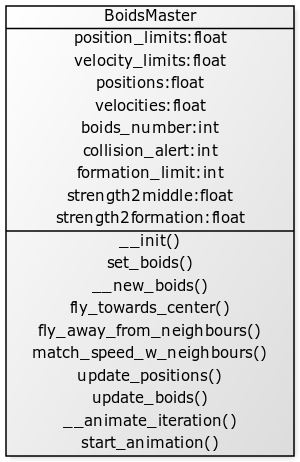
\includegraphics[height=3in]{uml_boids}%
\caption{ UML class design}
\label{fig:uml_design}
\end{figure*}
%%%%%%%%%%%%%%%%%%%%%%%%%%%%%%%%%%%%%%%%



%\problemAnswer{
%\begin{center}
%%\includegraphics[width=0.75\columnwidth]{example_figure} % Example image
%\end{center}
%
%\lipsum[3-5]
%}
\end{homeworkProblem}

%----------------------------------------------------------------------------------------

\begin{homeworkProblem}


\textbf{The advantages of a refactoring approach to improving code}\\

Refactoring is a way to make your code easier to understand and to follow. Strategies like breaking the code apart in small units that differ from each other based on functionality and creating variable names that explain the concepts, help other developers build on top of the project. Furthermore, a project that is well documented and refactored to be self-explanatory is much easier to debug. Refactoring can also speed up the coding process, since the developer does not need to spend time understanding the state of the project, because all the concepts are well embedded in the variable names.


\end{homeworkProblem}


%----------------------------------------------------------------------------------------

\begin{homeworkProblem}
  
\textbf{Discuss problems encountered during the project}\\

After each small change in the code, the regression test was run. After replacing the for loops of the functions for the behaviour of the flock (i.e. moving towards the center, flying in formation), the initial regression test failed with small differences (figure \ref{fig:regression_test}). This was ultimately solved by generating new fixtures for each case and using it as a regression test in the following refactoring process(figure \ref{fig:good_test}).

%%%%%%%%%%%%%%%%%%%%%%%%%%%%%%%%%%%%%%%%
\begin{figure*}[!h]
\centering
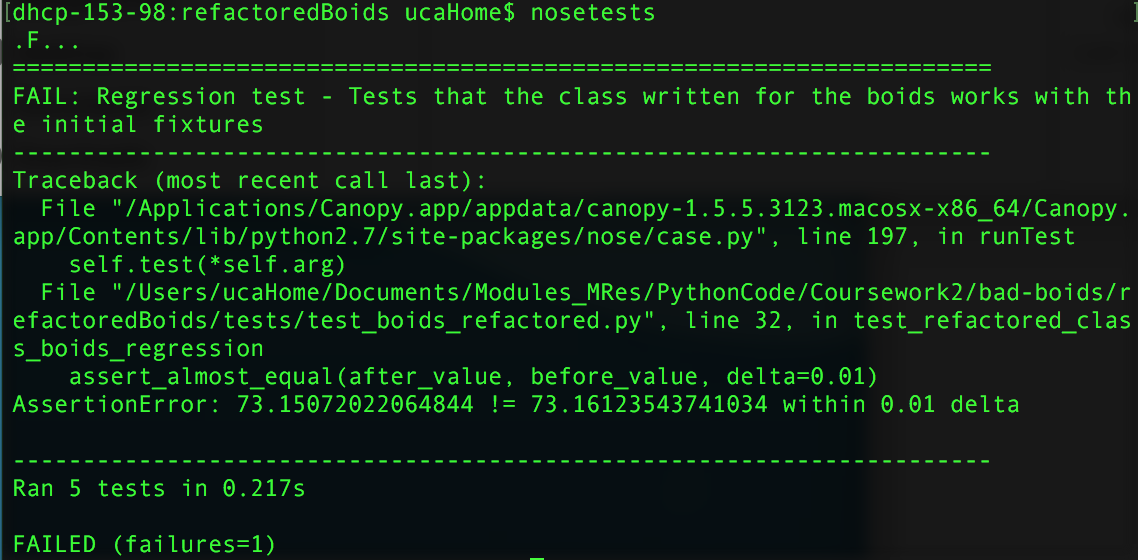
\includegraphics[height=3in]{regressiontest_fail}%
\caption{Failed regression test}
\label{fig:regression_test}
\end{figure*}
%%%%%%%%%%%%%%%%%%%%%%%%%%%%%%%%%%%%%%%%
%%%%%%%%%%%%%%%%%%%%%%%%%%%%%%%%%%%%%%%%
\begin{figure*}[!h]
\centering
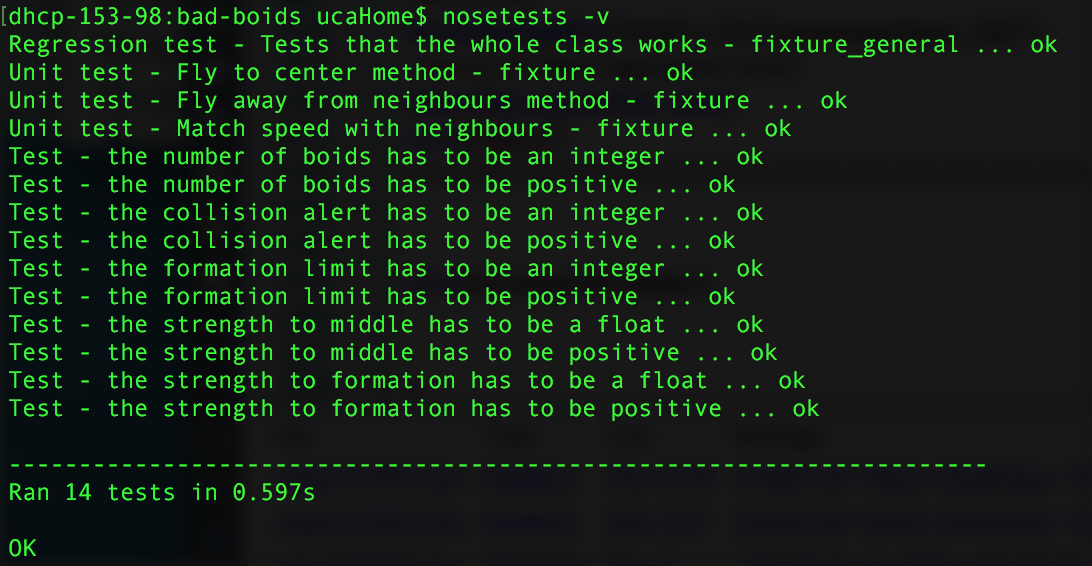
\includegraphics[height=3in]{tests_good}%
\caption{Final tests}
\label{fig:good_test}
\end{figure*}
%%%%%%%%%%%%%%%%%%%%%%%%%%%%%%%%%%%%%%%%

\end{homeworkProblem}


%----------------------------------------------------------------------------------------

\end{document}